% DRAFT supplementary subsection: prior sensitivity of Model 2a.
% Artifacts (generated by prior_sensitivity.py):
%   \begin{tabular}{lrccc}
\toprule
Prior scenario & $\hat{k}$ & $\pi$ (median wt) & Handling, warm 6\,wk (min) & Warmed$\times$6\,wk coef. \\
\midrule
Primary prior & 0.00 & 0.94 [0.91, 0.96] & 7.90 [7.13, 8.74] & -0.74 [-0.88, -0.61] \\
$\gamma_0$ mean $-2$ & -0.27 & 0.94 [0.91, 0.96] & 7.90 [7.12, 8.74] & -0.74 [-0.88, -0.61] \\
$\gamma_0$ mean $0$ & -0.10 & 0.94 [0.91, 0.96] & 7.91 [7.13, 8.75] & -0.74 [-0.88, -0.61] \\
$\gamma$ sd $2.5$ & 0.06 & 0.94 [0.92, 0.96] & 7.91 [7.13, 8.75] & -0.75 [-0.88, -0.61] \\
Slope sd $3/\sqrt{p}$ & 0.51 & 0.94 [0.92, 0.96] & 7.96 [7.27, 8.85] & -0.86 [-0.98, -0.73] \\
$c_r$ sd $1.0$ & -0.10 & 0.94 [0.91, 0.96] & 7.91 [7.13, 8.75] & -0.75 [-0.88, -0.61] \\
$c_r$ mean $\log 10$ & -0.11 & 0.94 [0.91, 0.96] & 7.92 [7.13, 8.76] & -0.75 [-0.88, -0.61] \\
$c_r$ mean $\log 30$ & -0.31 & 0.94 [0.91, 0.96] & 7.89 [7.12, 8.73] & -0.74 [-0.88, -0.61] \\
All widened & 0.41 & 0.94 [0.92, 0.96] & 8.00 [7.27, 9.01] & -0.86 [-0.98, -0.74] \\
\bottomrule
\end{tabular}

%   figures/sensitivity_panelA.png, figures/sensitivity_panelB.png
% (full weighted summaries in outputs/sensitivity/sensitivity_summary.csv)

\subsection{Prior sensitivity}
\label{supp:prior_sensitivity}

We assessed how the conclusions of the selected model (All-$h$ + voracious
mixture) depend on the choice of prior. Because refitting under many priors is
expensive, we used Pareto-smoothed importance sampling (PSIS): each posterior draw
from the primary fit was reweighted by the ratio of an alternative prior to the
primary prior, $w_i \propto p_{\text{new}}(\theta_i)/p_{\text{old}}(\theta_i)$,
and quantities of interest were recomputed as weighted posterior summaries
\citep{vehtariPracticalBayesianModel2017}. Reweighting is reliable when the
estimated Pareto shape $\hat{k} < 0.7$. We considered only priors that
\emph{widen} or \emph{shift} the primary prior (never narrow it): shifting the
mixture intercept $\gamma_0$ so that the prior mean voracious probability is as low
as $\approx 0.12$ or as high as $0.5$; widening the mixture-prior scale; widening
the regression-coefficient scale fourfold (to $3/\sqrt{p}$); widening and shifting
the handling-rate intercept prior $c_r$; and a joint ``all widened'' prior. All
scenarios satisfied $\hat{k} < 0.7$.

The results were highly robust (Table~\ref{supp:tab_prior_sens}). The estimated
voracious fraction was essentially unchanged across every scenario---median-weight
$\pi \approx 0.94$ ($95\%$ CI $\approx 0.91$--$0.96$) even when the prior mean was
moved to $0.12$ or $0.5$---confirming that this quantity is determined by the data
rather than the prior. The treatment effects on handling time were similarly
stable: reproducing Figure~\ref{fig:fig3}A,B under every prior
(Figs.~\ref{supp:sensA}--\ref{supp:sensB}) gives visually indistinguishable
patterns. The only appreciable movement occurred under the fourfold
coefficient-widening (and the ``all widened'' prior), which---by imposing less
shrinkage---slightly \emph{strengthened} the treatment effects (e.g.\ the
warmed $\times$ 6-week interaction coefficient moved from $-0.74$ to $-0.86$, and
the warmed 6-week handling time from $7.9$ to $8.0$~min) without changing their
sign or interpretation. We therefore conclude that the substantive findings are
not artefacts of the prior specification.

\begin{table}[h]\centering
\caption{Prior sensitivity of Model 2a under widened/shifted priors, via PSIS
reweighting (no refit). $\hat{k}$ is the Pareto diagnostic ($<0.7$ throughout,
so reweighting is reliable); entries are weighted posterior medians with $95\%$
credible intervals. Full summaries are in \texttt{sensitivity\_summary.csv}.
\label{supp:tab_prior_sens}}
\begin{tabular}{lrccc}
\toprule
Prior scenario & $\hat{k}$ & $\pi$ (median wt) & Handling, warm 6\,wk (min) & Warmed$\times$6\,wk coef. \\
\midrule
Primary prior & 0.00 & 0.94 [0.91, 0.96] & 7.90 [7.13, 8.74] & -0.74 [-0.88, -0.61] \\
$\gamma_0$ mean $-2$ & -0.27 & 0.94 [0.91, 0.96] & 7.90 [7.12, 8.74] & -0.74 [-0.88, -0.61] \\
$\gamma_0$ mean $0$ & -0.10 & 0.94 [0.91, 0.96] & 7.91 [7.13, 8.75] & -0.74 [-0.88, -0.61] \\
$\gamma$ sd $2.5$ & 0.06 & 0.94 [0.92, 0.96] & 7.91 [7.13, 8.75] & -0.75 [-0.88, -0.61] \\
Slope sd $3/\sqrt{p}$ & 0.51 & 0.94 [0.92, 0.96] & 7.96 [7.27, 8.85] & -0.86 [-0.98, -0.73] \\
$c_r$ sd $1.0$ & -0.10 & 0.94 [0.91, 0.96] & 7.91 [7.13, 8.75] & -0.75 [-0.88, -0.61] \\
$c_r$ mean $\log 10$ & -0.11 & 0.94 [0.91, 0.96] & 7.92 [7.13, 8.76] & -0.75 [-0.88, -0.61] \\
$c_r$ mean $\log 30$ & -0.31 & 0.94 [0.91, 0.96] & 7.89 [7.12, 8.73] & -0.74 [-0.88, -0.61] \\
All widened & 0.41 & 0.94 [0.92, 0.96] & 8.00 [7.27, 9.01] & -0.86 [-0.98, -0.74] \\
\bottomrule
\end{tabular}

\end{table}

\begin{figure}[h]\centering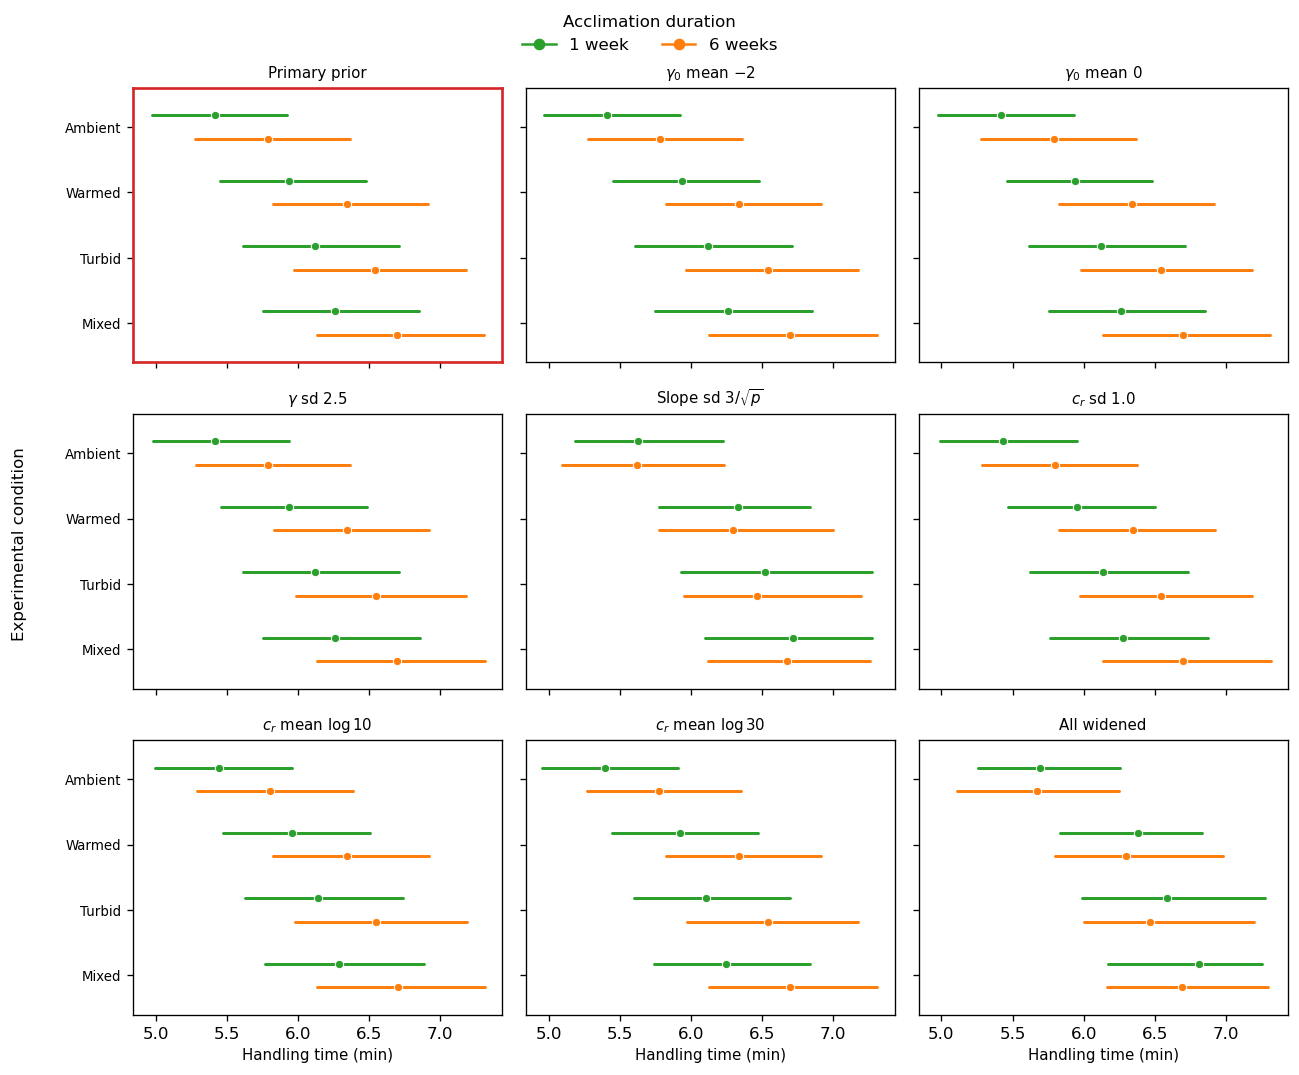
\includegraphics[width=\textwidth]{figures/sensitivity_panelA.png}
\caption{Figure~\ref{fig:fig3}A (handling time by experimental condition,
acclimation held at Ambient) reproduced under each prior scenario; the primary
prior is outlined in red. Points are posterior medians, whiskers $95\%$ intervals.
\label{supp:sensA}}\end{figure}

\begin{figure}[h]\centering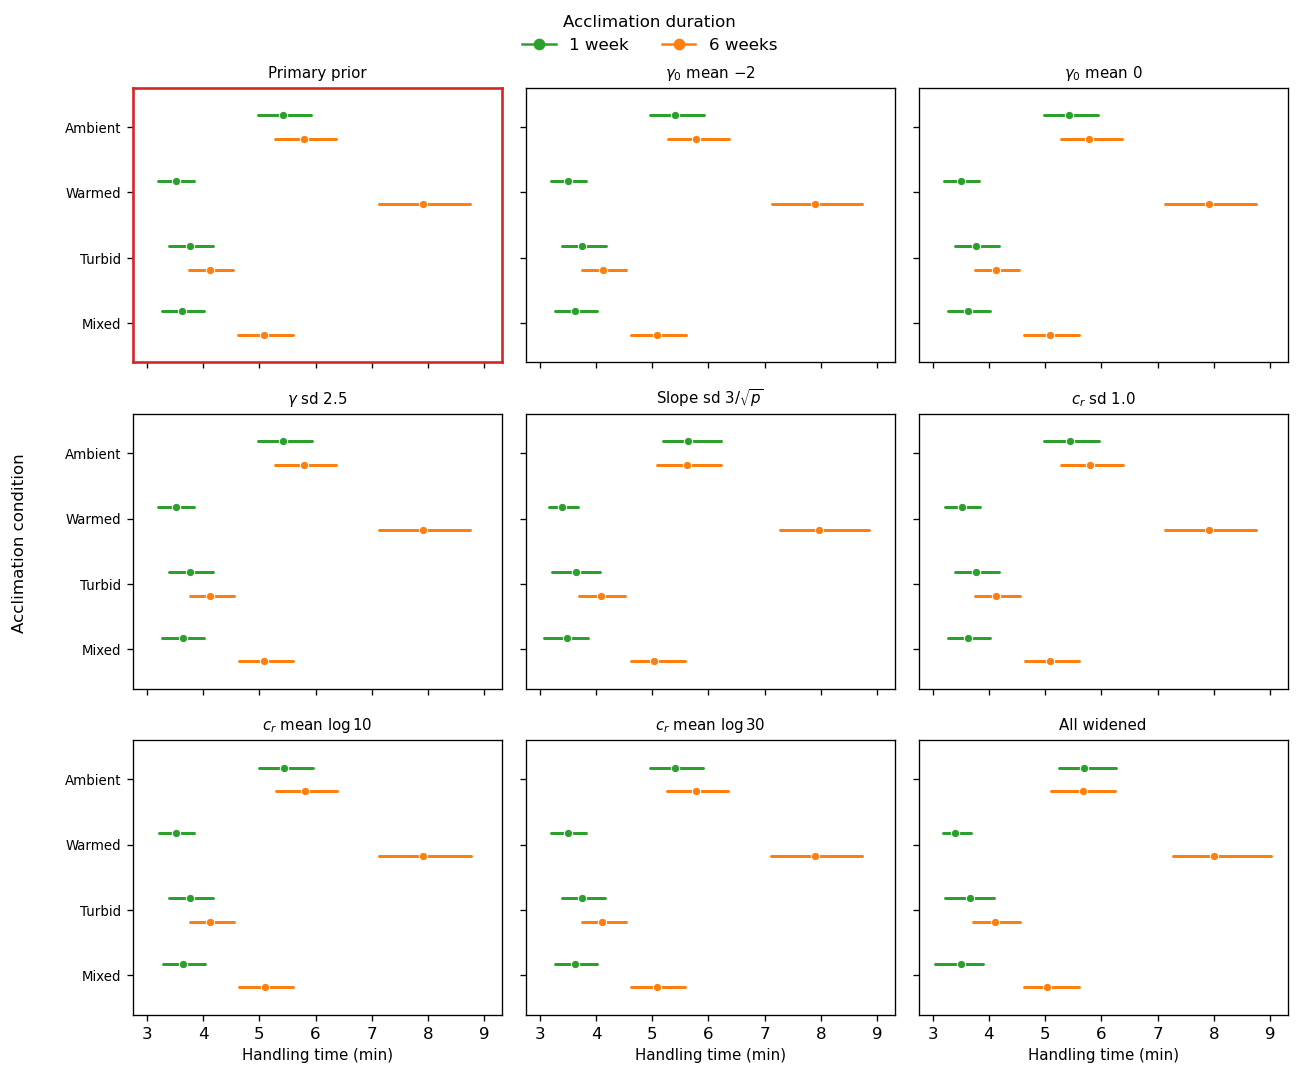
\includegraphics[width=\textwidth]{figures/sensitivity_panelB.png}
\caption{Figure~\ref{fig:fig3}B (handling time by acclimation condition,
experiment held at Ambient) reproduced under each prior scenario; the primary
prior is outlined in red. Points are posterior medians, whiskers $95\%$ intervals.
\label{supp:sensB}}\end{figure}
